We show that the proposed rewriting leads to better performance in a large variety of "real-world" data analytics scenarios. In this section, we present an abstract analysis of the cost of the TAAT, NSAAT and DSAAT algebraic formulations on execution environments typically utilized for those scenarios. For this purpose, we introduce a theoretical cost model focused on network overhead and disk access  based on a number of (listed) assumptions regarding network, storage, indices and relational operators which are common across those execution environments.

\begin{figure}[h]
\centering
\caption{Query Processor Architecture \label{fig:architecture}}
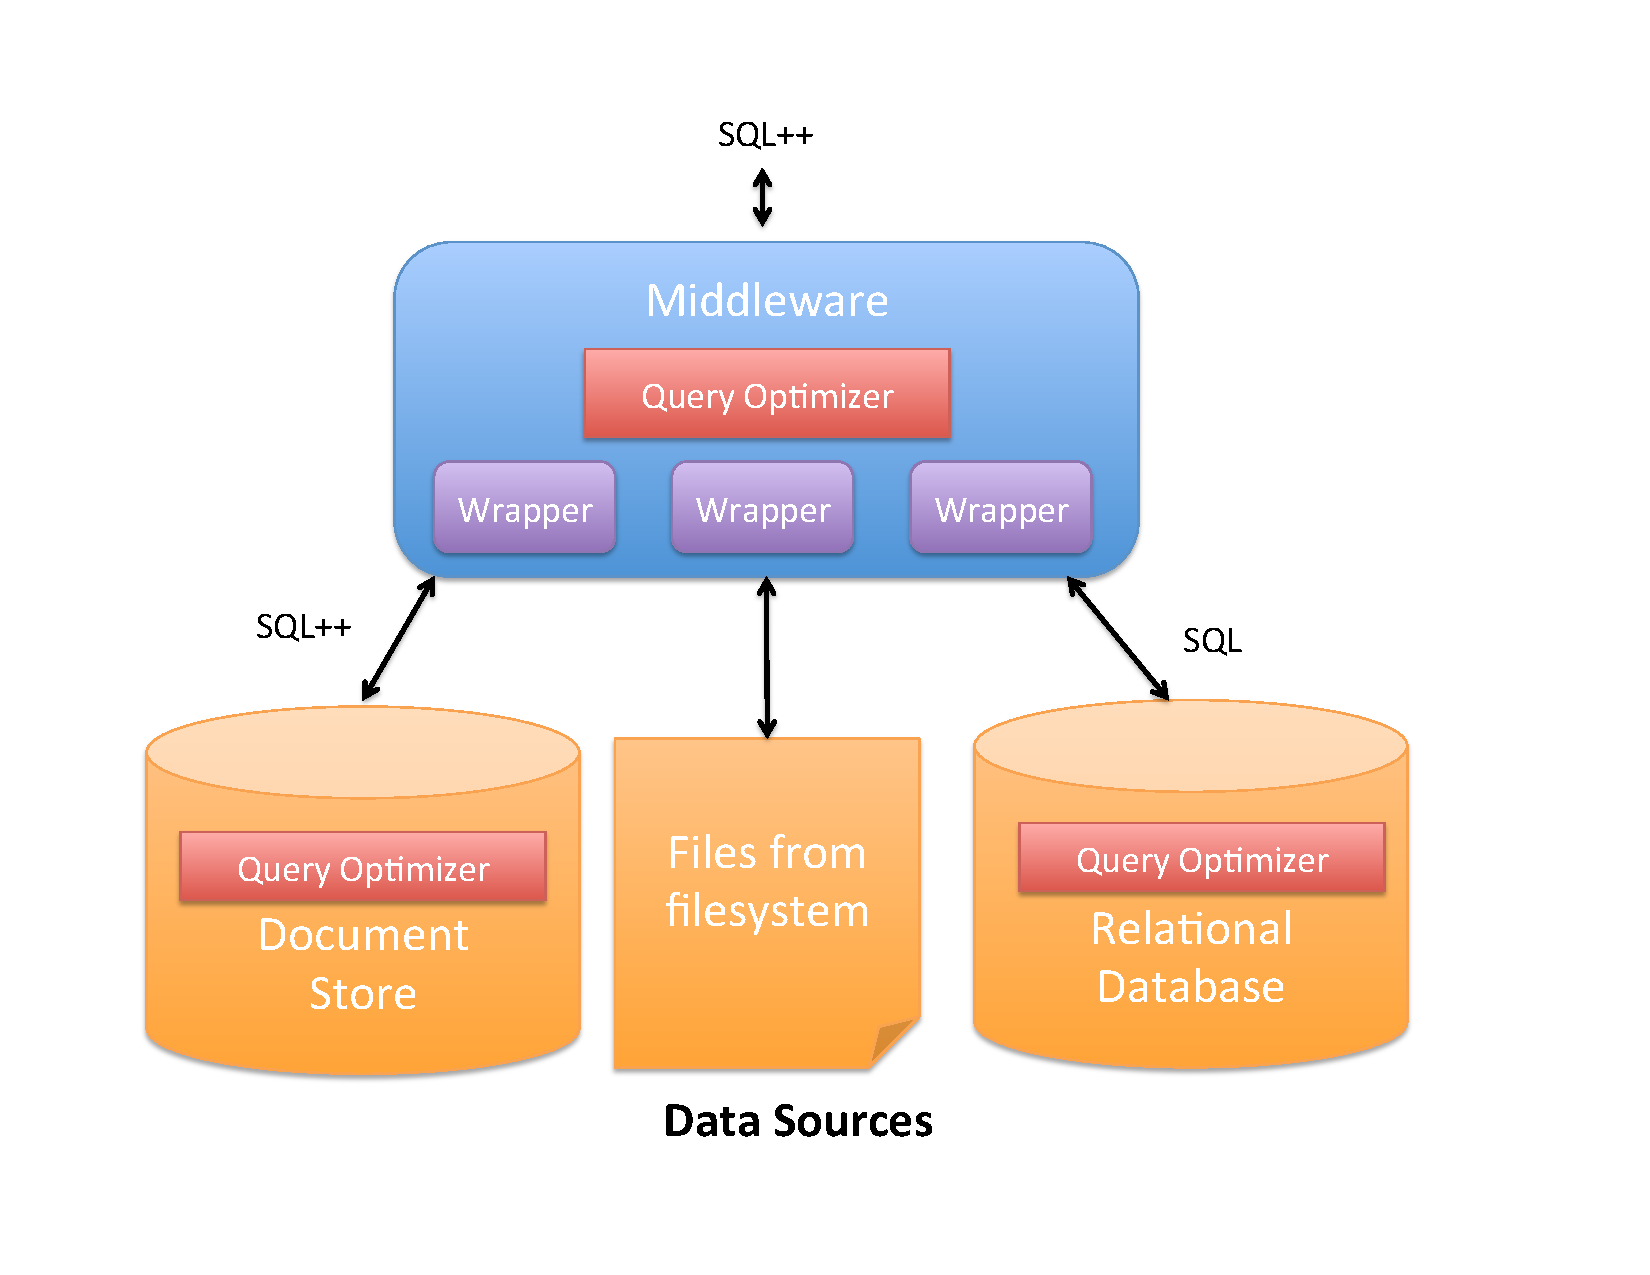
\includegraphics[width=\linewidth]{images/Architecture.pdf}
\end{figure}

\subsection{Setup}

\subsubsection{Execution Environment}

We argue the query rewriting presented in this paper has value on a variety of different query processors for semi-structured data. We consider two broad categories of query processors: document stores and data integration middlewares. We evaluate the performance improvement of our rewriting using a theoretical architecture (shown on figure \ref{fig:architecture}) which is representative of both categories. This architecture has two components: a data processing \emph{middleware}, and a set of zero or more \emph{data sources} with various levels of \emph{capabilities}.

\textbf{Middleware}: the data processing middleware answers SQL++ queries by executing algebraic plans over the data sources. It is capable of processing any SQL++ algebraic operator. To process SQL++ algebraic operators, the middleware has access to a number of physical operators (algorithms) which are listed on table \ref{table:op-costs}. The middleware also has access to a query optimizer, which allows it to choose which physical implementation to use for processing of a given algebraic operator. It is also capable of delegating a portion or all of the plan to a data source, if : 1) the data source is capable of processing all operators in that plan and 2) all stored collections accessed in that plan are located at that data source. Once a plan is delegated to a datasource, the wrapper for that datasource converts the algebraic plan into a query expressed in that datasource's native query language.

\textbf{Data Sources}: they contain the data queried by the middleware. We consider here only three kinds of data sources: a file system, a traditional relational database system and document stores. Each data source has its own set of characteristics which we describe next:

\begin{itemize}
\item{\textbf{File System}: Any file system which is accessible by the middleware process. This source is not capable of processing any SQL++ operator.}
\item{\textbf{RDBMS}: Any relational database system which has access to the physical operators shown on table \ref{table:op-costs}. For simplicity, we do not assume the RDBMS has access to any other physical operators. An RDBMS is only capable of processing \emph{purely relational} operators. By purely relational, we mean operators whose output are regular rows of atomic scalars (i.e. they do not contain any nesting or heterogeneity).}
\item{\textbf{Document Store}: we consider any document store which is capable of processing any SQL++ algrebraic plan. We assume the document store  also has access to the physical operators shown on table \ref{table:op-costs}. In the case where the document store is the single datasource, we consider the middleware optional (the user may query using the document store directly).}
\end{itemize} 

We assume that all query processors considered to be using single machine setups. We do not consider the cases where operators can run as parallel tasks of a cluster in a share-nothing architecture. We also assume all databases (including the middleware) have the ability to spill to disk in case the size of an intermediate results exceeds the available memory. In practice, document stores as well as integration middlewares employ complex optimizations that cannot be comprehensively accounted for in an analytical model. As such, the computation costs and associated speedups reported in this section should be used as rough estimates of the actual cost.

The middleware answers queries from a single source at a time (i.e. we do not consider complex cases where the data is joined from multiple source in the middleware). This assumption is of particular importance when 

\jules{@Yannis: I see a problem here when we reach experiments. I only know two kinds of middlewares (FORWARD middleware and Informatica), none of which can spill to disk without invoking a "supporting" database.}

\subsubsection{Notations}

\begin{itemize}
\item A plan context $P[]$ denotes a plan with one "hole"; i.e. a plan in which an $n$-ary operator has $n-1$ operators and a special character $[]$ as children, and $P[Q]$ represents the plan $P$ in which the hole has been replaced with the subplan $Q$. For example, for $P[] = \pi_p([])$ and $Q = \sigma_w(R)$, we have $P[Q] = \pi_p(\sigma_w(R))$.
\item $cost(P)$ denotes the cost of executing a plan $P$ and $cost(P[],Q)$ denotes the cost of executing the plan $P[Q]$ assuming $Q$ has already been evaluated and its result is accessible is accessible at no cost.
\item $network(P)$ denotes the cost of sending the result of $P$ to a target database system through a network with throughput $K_n$. Notice that we only consider "internal" network cost. For example, in the Hadoop ETL setting, we do not consider the cost of sending the end result to the target database. 
\item $|P|$ denotes the number (resp. average number) of binding tuples outputted by a subplan (resp. correlated subplan) $P$. Conversely $\#_f(P)$ is the number (resp. average number) of memory frames required to store the result of subplan (resp. correlated subplan) $P$. Thus we have $\#_f (E) = \ceil{\frac{|E|.T_E}{f_s}}$, where $T_E$ is the tuple width and $f_s$ is the frame size. In the remaining of the paper, we approximate this expression to $\#_f(E) = \frac{|E|}{f_s}$. \jules{This approximation could cause a problem, since tuples containing nested collections may have arbitrary size and ignoring this can lead to incorrect size estimates. Likewise, one of the advantages of NSAAT over DSAAT is the decrease in tuple width, which this assumption would eliminate.}
\item $attr(E)$ denotes the set of attributes in the output of expression $E$.
\item $join\_size(E,F,w)$ denotes the size of the output (in memory frames) of a join with condition $w$. We have $(E,F,e.c = f.c \cap w')) = \#_f \frac{|E| |F|}{max(V(c,E),V(c,F))} s_{w'}$, where $c \in attr(E) \cap attr(F)$ and $s_{w'}$ is the selectivity of the condition $w'$. Notice that we do not distinguish between the size of the output of an inner and the outer join.
% \item Denote $R_g$ the group of tuples in the output of $R$ with grouping attribute values equal to $g$ for some $g$.
\item Aggregation functions are said to be $bounded-state$ if the size of their output is bounded. Traditional aggregation functions such as \texttt{COUNT(.)} and \texttt{AVERAGE(.)} belong to this category, while \texttt{NEST(.)} does not, since the size of its output grows with the size of its input.
\item We denote $M_{DB}$ as the memory budget for each operator in database system $DB$ (e.g. $M_{PostgreSQL}$ when considering the PostgreSQL system). This memory budget is expressed in terms of number of memory frames. We assume all operators in a given database system are entitled to the same memory budget. In cases where there is only one database system for an execution environment, we simply say $M$.
\item We denote $V(c,E)$ as the number of distinct values of attribute $c$ in the output of expression $E$.
\item We call the \emph{reach} of a query the amount of data which \emph{must} be read from database instance in order to accurately answer a query, while in the presence of all possible indices.\jules{I would be surprised if I am the first to ever introduce this term.}
\item We denote $merge(R)$ as the cost of sorting using the merge-sort join technique beyond the first pass.  Note that $merge(R) = \#_f(R)$ when $R < M^2$ (only two passes).
\end{itemize}

\begin{table*}[t]
\centering
\caption{Operator Costs \label{table:op-costs}}
\begin{tabular}{|c|C{2.5cm}|C{3cm}|C{2.5cm}|C{3cm}|}
\hline
Physical Operator / Color Code & Read Cost & Transform Cost & Write Cost  & Restrictions / Characteristics \\ \hline
$ T \leftarrow R$ (Copy) & $\#_f(R)$ & 0 & $\#_f(R)$ &  \\ \hline
$\sigma_w, \pi_p, \lambda_l$ &  0 &  0 & 0  & pipelined  \\ \hline
$ Scan^{\textbf{sequential}}(R)$ & $\#_f(R)$ & 0 & 0 & \\ \hline
$ Scan^{\textbf{index}}_{c_r = X}(R)$ & $\frac{|R|}{V(c,R)}$ & 0 & $\#_f(\frac{|R|}{V(c,R)})$ & $R$ is a table, $c_r \in attr(R)$, index on $R.c$ and $X$ is a scalar  \\ \hline
$Join^{\textbf{memory\_hash}}_{c_r = c_s}(R,S)$ & $ \#_f(S) + \#_f(R)$ & 0 & $join\_size(R,S,w)$ & $\#_f(R) < M_{DB}$, $R$ already loaded in memory  \\ \hline
$Join^{\textbf{right\_index}}_{c_r = c_s}(R,S)$ & $\#_f(R)$ & $|R| \frac{|S|}{V(c,S)}$ & $join\_size(R,S,w)$ & $\#_f(R) < M_{DB}$, $R$ already loaded in memory   \\ \hline
$Join^{\textbf{sort\_merge}}_{c_r = c_s}(R,S)$ & $\#_f(R) + \#_f(S)$ & $\#_f(R) + \#_f(S) + merge(R) + merge(S)$ & $join\_size(R,S,w)$ &   \\ \hline
$Join^{\textbf{sort\_merge}}_{c_r = c_s}(R,S)$ & $merge(R) + merge(S)$ & 0 & $join\_size(R,S,w)$ & inputs $R$ and $S$ are sorted on join attributes  \\ \hline
% $Join^{reduce-side}_{c_r = c_s}(R,S)$ & ? & ? &  $join\_size(R,S,w)$ & ?  & H  \\ \hline
% $Join^{map-side}_{c_r = c_s}(R,S)$ & ? & ? &   $join\_size(R,S,w)$ & ? &  H \\ \hline
$\tau(R), \chi(R), \gamma_{NEST}^{\textbf{SB}}(R)$ & $\#_f(R)$ & $\#_f(R) + merge(R)$ & $\#_f(R)$  &   \\ \hline
$\gamma_{NEST}^{\textbf{PC}}(R)$ & $\#_f(R)$ & 0 &  $\#_f(R)$ & input $R$ is sorted on $g$  \\ \hline
$\gamma_{BS}^{\textbf{PC}}(R), \delta_{PC}(R)$ & $\#_f(R)$ &  0 & $\#_f(\delta(\pi_g(R))$ & input $R$ is sorted on $g$ \\ \hline
$\gamma_{BS}^{\textbf{SB}}(R), \delta_{SB}(R)$ & $\#_f(R)$  & $\#_f(\delta(\pi_g(R)) + merge(R)$ & $\#_f(\delta(\pi_g(R))$ &   \\ \hline
$\alpha_{P \rightarrow N}(R)$ & $\#_f(R)$ & $|R| cost(P)$ & $\#_f(R)$ & Tuple size increased, number of tuples reduced  \\ \hline
\end{tabular}
\end{table*}

\subsubsection{Assumptions}

To make the analysis simpler, we first make the following assumptions (and discuss them later on):

\begin{itemize}
\item We assume the size of a memory frame $\#_f(F)$ equals the size of a disk block.  This way we have $SeqScan(R) = \ceil{\frac{R.T_R}{B}} = \ceil{\frac{R.T_R}{f_s}} = \#_f(R)$.
\item We only look at the number of blocks, not at the time required to fetch those blocks (not distinguishing between random and sequential IO). 
\item We assume all indices are available and will be used by the query optimizer of the database system if it chooses to do so.
\item We assume no skew in correlation attribute values. This way, we assume that the value of attribute $N$ of a apply plan operator $\alpha_{P(c_1,\dots,c_n) \rightarrow N}$ will have the same size, no matter which values correlated attributes $c_1,\dots,c_n$ take.
\item We assume $\alpha_{P(c_1,\dots,c_n) \rightarrow N}$ are applied sequentially, with the fully memory budget available to \emph{each} execution of the plan $P$.
\item In all scenarios, we assume the size of the result of the inner query (of the query pattern, that is) is expected to be small, given that nesting big collections isn't practical and does not represent a real use case.
\item The \texttt{FROM} clause $F$ of the inner plan $P$ is a join of $n$ stored collections. We assume only one of these collections, denoted with $R$, is correlated with the outer plan through a selection $\sigma_{c_e = c_r}(R)$, where $c_e$ and $c_r$ attributes of $E$ and $R$, respectively. We denote $F'$ the plan context such that $F = F'[\sigma_{c_e = c_r}(R)]$. Finally the expression $rf(F,T)$ is such that the join order of $F$ has not changed. That is, $rf(F,T) = F'[T \innerjoin_{c_e = c_r} R]$.
\item We assume the presence of both \texttt{GROUP BY} and \texttt{ORDER BY} clause in the input nested query. \jules{@Yannis: I believe it is not necessary to explicitly describe queries with either only \texttt{GROUP BY} or only \texttt{ORDER BY} in the nested query separately.}
\item We make the assumption that $\frac{|F|}{M f_s} \leqslant f_s$, which is true anytime $|F|$ is smaller than $f_s$ times the memory size. Given $f_s$ typically ranges in the kB to MB range, this assumption holds unless $|F|$ is bigger than one million times the memory size, which we don't consider realistic in practice.
\item We make the assumption that no stored collection or intermediate result ever exceed $M^2$, which reflects realistic use cases.
\item In the case of an index being used by a $Scan^{index}$ or $Join^{right\_index}$ operator, we assume this index is stored entirely in memory, and does not take space in the memory budget allocated for the query.
\end{itemize}

Note that the running example query follows these assumptions.

\subsubsection{Operators considered}

Our cost model provides a taxonomy of physical operators implementations which can be used to form execution plans (those are shown on table \ref{table:op-costs}). Each row on table \ref{table:op-costs} corresponds to a implementation of a algebraic operator. The cost associated with using this operator is split into three sections: read cost, transform cost and write cost. Write cost is only paid if output is too large to fit in memory and is not the final result. Read cost is paid if input is not already in memory. In case of joins, if one of the inputs is already in memory but not both, then only the cost of reading the input not in memory is paid. Transform cost is paid if size of the input is greater than memory. The cost of the execution of a given operator is the sum of all three costs. Finally, the restrictions column indicates under which conditions can a particular implementation be used. Therefore, we define the \emph{cost} of executing an algebraic operator to be the cheapest cost among competing implementations of that operators which meet the restrictions. 

\subsubsection{Cost Breakdowns}

We next describe precisely the cost breakdown of expressions TAAT, NSAAT and DSAAT. 

\eat{
We assume the SQL++ queries being evaluated exhibit the following pattern :
\lstinputlisting[language=SQL]{code/query_pattern.sql}
Note that within the nested query, we assume presence of both \textt{GROUP BY} and \texttt{ORDER BY} clause. 
}

\begin{equation*}
\begin{aligned}
cost(TAAT) = & |E| (cost(Scan(R)) + cost(F'([]), Scan(R)) + \\
                    & + cost(\tau(\gamma_{inner}([])), F)) \\
\end{aligned}
\end{equation*}

The TAAT plan evaluates $|E|$ times the inner plan $P$, which itself is the addition of the following costs: i) the cost of evaluating the \texttt{FROM} clause (which requires scanning collection $\sigma_{e_c = r_c}(R)$ and joining with other collection in plan context $F'$) and ii) the cost of evaluating the inner \texttt{GROUP BY} (denoted $\gamma_{inner}$) and \texttt{ORDER BY} clauses on the output of the \texttt{FROM} clause.

\begin{equation*}
\begin{aligned}
cost(NSAAT) = & cost(E \rightarrow T) + cost(rf(F,T))   \\
                    & + cost(\gamma_{\texttt{NEST}}(\chi(\gamma_{inner}([])), rf(F,T)) \\
                    & + cost(\leftouterjoin([T,]),r(P,T))  \\
\end{aligned}
\end{equation*}

The cost of evaluating the NSAAT plan is the addition of the following costs : i) the cost of the assignment $E \rightarrow T$ ii) the cost of evaluating $rf(F,T)$ iii) the cost of the $\gamma_{inner}$ aggregation, the $\chi$ partition-based ordering and the $\gamma_{\texttt{NEST}}$ nesting aggregation iv) the cost of the final outer join between $T$ and $r(P,T)$. Note that evaluating $rf(F,T)$ requires performing an inner join between the distinct correlated values fetched from $T$ and the expression $F$ resulting in a the following cost : $cost(rf(F,T)) = cost(\delta(T)) + cost(\innerjoin([,R]),\delta(T)) + cost(F'([]), \innerjoin(\dots))$. 

\begin{equation*}
\begin{aligned}
cost(DSAAT) = & cost(F) + cost(\leftouterjoin([E,]),F) \\
                   & + cost(\gamma_{\texttt{NEST}}\chi(\gamma_{inner}([])), \leftouterjoin(
                   \dots)) \\
\end{aligned}
\end{equation*}

Finally, the cost of evaluating the DSAAT plan is the addition of the following costs: i) the cost of expression $F$, ii) the cost of the initial outer join between $E$ and $F$ iii) the cost of the $\gamma_{inner}$ aggregation, the $\chi$ partition-based ordering as well as the $\gamma_{\texttt{NEST}}$ aggregation.

Note that these costs assume that selection pushdown and cross-product removal optimizations have already occurred. Given the cost of computing expression $E$ is paid no matter what, it is not included in the above cost expressions. Note as well that pipelined operators ($\lambda$, $\sigma$ and $\pi$) are not included either. Finally, some systems may introduce additional costs to those expressions, such as network costs in middleware settings.

\subsection{Scenarios}

We next evaluate the performance of the TAAT, NSAAT and DSAAT algebraic formulations in three different scenarios.  For each scenario, we describe the characteristics of the query pattern and then discuss and compare the cost of the expressions for different ranges of $V(c_e,E)$ and $V(c_r,F)$, the number of distinct correlated attribute values for expressions $E$ and $F$, respectively. Finally, we summarize the cheapest implementations for each scenario in the appendix cost tables \ref{table:r0}, \ref{table:r2} and \ref{table:r4}.

\subsubsection{Scenario 1: Large Reach, Small Output}

This situation is typical of analytical intelligence use cases, in which human analysts query large datasets and read the results of their queries to obtain valuable insight. The running example scenario belongs to this category. 

\begin{itemize}
\item{The result of such use cases are typically small (thus the "small output"), since they have to be human-readable. As a result, the size of $E$ is expected to be tiny in database terms (may be less than 100). In this situation, the cost $E \rightarrow T$, $\delta(T)$ and $\gamma_{\texttt{NEST}}$ are insignificant.}
\item {The expression $F$ could be very large (thus the "large reach"), and exceed the memory budget $M$ many times.}
\end{itemize}

\subsubsection{Scenario 2: Large Reach, Large Output}

This situation is typical of ETL use cases, in which large datasets are transformed and loaded into semi-structured databases. 

\begin{itemize}
\item{The aim of such use cases is too transform large quantities of data in a single query. The result of such use cases may be well beyond a human readable size. As a result, the size of $E$ is expected to be very large. In this situation, the cost $E \rightarrow T$, $\delta(T)$ and $\gamma_{\texttt{NEST}}$ become significant.}
\item {The expression $F$ could be very large (thus the "large reach"), and exceed the memory budget $M$ many times.}
\end{itemize}

\begin{figure*}[h]
\centering
\caption{Physical Query Plans \label{fig:plans}}
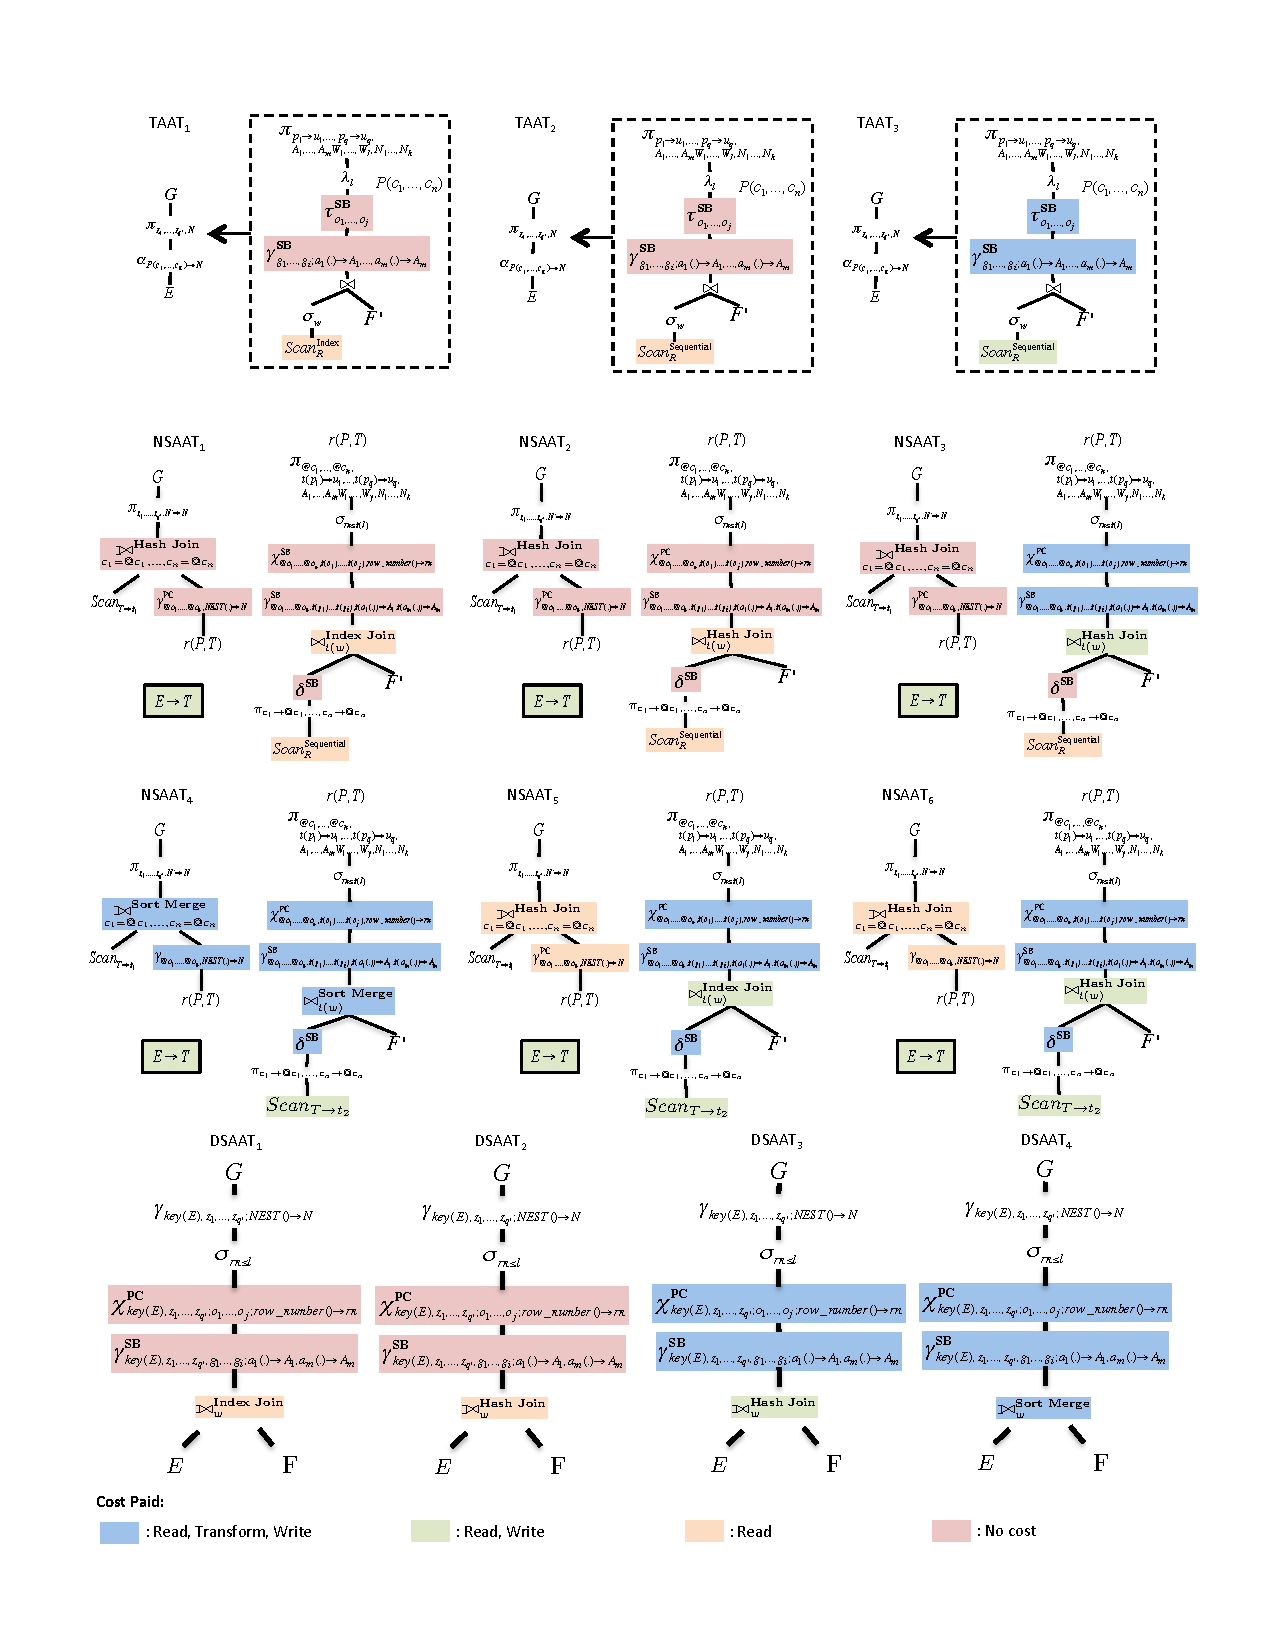
\includegraphics[width=\linewidth]{images/PhysicalPlans.pdf}
\end{figure*}

\subsection{Document Store}

The physical plans produced by the query optimizer for each formulation are shown on figure X.

\subsubsection{Scenario 1}

\subsubsection{Scenario 2}

\subsection{Middleware}

\subsubsection{Scenario 1}

\subsubsection{Scenario 2}

\jules{Index join is only if possible if $n$ is 1}

\eat{
\textbf{Discussion}: on figure \ref{fig:scenario1} of appendix \ref{app:cost}, we display the cost of each formulation for different ranges of $V(c_r,F)$ (number of distinct correlated attribute values), assuming the query optimizer picks the cheapest option for every operator. All values within the same range result in the same physical implementations being chosen as by the query optimizer. We discuss specific ranges further:

% Discuss borders
\begin{itemize}
\item When $f_s \leqslant V(c_r,F)$,  expressions $\sigma_{c_e=c_r}(F)$ and $\innerjoin_{c_e=c_r}(E,F)$ have high selectivity and small output, resulting in the use of index joins/scans and in-memory sorting for all subsequent $\gamma$, $\tau$ and $\chi$ operations. In this situation, TAAT loses big given the cost of $F'$ may be significant, since $F'$ would has to be paid $|E|$ times more than on NSAAT, DSAAT. NSAAT is cheaper than DSAAT, but only marginally, because NSAAT's index join is executed on fewer tuples than DSAAT's. \textbf{Result}: NSAAT < DSAAT < TAAT.
% Otherwise, costs for all expressions are roughly the same, since $V(c,E) \simeq |E|$ when $E$ is small.
\item When $V(c,F) \leqslant \frac{|F|}{M f_s}$: expressions $\sigma_{c_e=c_r}(F)$ and $\innerjoin_{c_e=c_f}(E,F)$ are not selective and have even larger outputs, which results in sequential scans or hash-joins being used, as well as external sorting. In this situation, TAAT is the most expensive, while NSAAT is only marginally cheaper than DSAAT, again due to $V(c,E) \simeq |E|$. \textbf{Result}: NSAAT < DSAAT < TAAT.
\item When $\frac{|F|}{M f_s} \leqslant V(c,F) \leqslant f_s$: the cheapest formulation depends on the parameters found on figure \ref{fig:scenario1}. Of particular interest are the boundaries $\frac{|F|}{M f_s}$, $\frac{V(c_e,E)|F|}{M f_s}$ and $\frac{|E||F|}{M f_s}$, which determine whether a formulation can rely on in-memory sorting or has to resort to an external sort to process the \texttt{GROUP BY} and \texttt{ORDER BY} clauses. In particular, the TAAT formulation can rely on in-memory sorting for lower values of $V(c_r, F)$. This is possible because of the following: while the TAAT formulation has to sort $|E|$ times, each result to be sorted is $|E|$ times smaller than in its set-at-a-time counterparts.
\end{itemize}
}
